Before we start to deduce all formulas of the GM-PHD filter, we should make several additional assumptions for the Gaussian-linear case in addition to the general ones given in Section \ref{sec:phd-filter-formal}:

\begin{enumerate}
    \item All targets have a Gaussian-linear single-target motion and measurement models, that is:

    \begin{align}
        f_{k|k-1}(\vecat{x}{k} | \vecat{x}{k-1}) &= \mathscr{N}\left(\vecat{x}{k}; \vecat{F}{k-1} \vecat{x}{k-1}, \vecat{Q}{k-1}\right), \\
        g_{k}(\vecat{z}{k} | \vecat{x}{k}) &= \mathscr{N}\left(\vecat{z}{k}; \vecat{H}{k}\vecat{x}{k}, \vecat{R}{k}\right),
    \end{align}

    \noindent where the detailed explanation of the meaning of $\vecat{F}{k-1}, \vecat{Q}{k-1}, \vecat{H}{k}, \vecat{R}{k}$ are given in Section \ref{sec:state-space}.
    
    \item Both the survival and detection probabilities are constant in time\footnote{A closed-form solution can be derived without this assumption, see Section III-E in \cite{voGaussianMixtureProbability2006}.}, that is, they do not depend on states:

    \begin{align}
        P_{S, k}(\vecat{x}{k-1}) &= P_{S, k},\\
        P_{D, k}(\vecat{x}{k}) &= P_{D, k}.
    \end{align}

    \item The birth intensity is modeled using a Gaussian mixture of the form:

    \begin{equation}\label{eq:gm-phd-birth-gm}
        \gamma_k(\vecat{x}{k-1}) = \sum_{i=1}^{J_{\gamma, k}} w_{\gamma, k}^{(i)}
        \mathscr{N}\left(\vecat{x}{k-1}; \vecat{m}{\gamma, k}^{(i)}, \vecat{P}{\gamma, k}^{(i)}\right),
    \end{equation}

    \noindent where $J_{\gamma, k}$ denotes the number of birth components, and $\vecat{m}{\gamma, k}^{(i)}$ and $\vecat{P}{\gamma, k}^{(i)}$ are the mean vector and the covariance matrix of each component. These are given as parameters and specified in advance according to the problem domain. Since this mixture is not a probability density by an intensity function, weights do not need to sum to one, and the weights $w_{\gamma, k}^{(i)}$ here represent the expected number of new targets that are expected to appear in a location centered at $\vecat{m}{\gamma, k}^{(i)}$.
\end{enumerate}

These assumptions form the basis for the Gaussian-linear PHD filter recursion formulas. Assuming these assumptions hold for a given problem, and by following the PHD filter recursion equations from Theorem \ref{theorem:phd-recursion}, we propose the following theorem:

\begin{theorem}[The GM-PHD filter prediction]\label{theorem:gm-phd-prediction}
    Given that the posterior intensity of the previous time step $v_{k-1}(\vecat{x}{k-1} | Z_{1:k-1})$ is a Gaussian mixture of the form:

    \begin{equation}
        v_{k-1}(\vecat{x}{k-1} | Z_{1:k-1}) = \sum_{i=1}^{J_{k-1}}
        \mathscr{N}\left(\vecat{x}{k-1}; \vecat{m}{k-1}^{(i)}, \vecat{P}{k-1}^{(i)}\right),
    \end{equation}

    \noindent where every Gaussian component has a unique tag or label assigned to it, which forms the set of tags:

    \begin{equation}
        T_{k-1} = \{ T_{k-1}^{(1)}, \ldots, T_{k-1}^{(J_{k-1})} \}.
    \end{equation}

    \noindent Then the predicted intensity at time $k$ is also a Gaussian mixture, defined as:

    \begin{equation}
        v_{k|k-1}(\vecat{x}{k} | Z_{1:k-1}) = \gamma_k(\vecat{x}{k}) + v_{S, k|k-1}(\vecat{x}{k}),
    \end{equation}

    \noindent where $\gamma_k(\vecat{x}{k})$ is given in Equation \ref{eq:gm-phd-birth-gm} and $v_{S, k|k-1}(\vecat{x}{k})$ is the PHD function of survived targets given by:

    \begin{align}
        v_{S, k|k-1}(\vecat{x}{k})
        &= P_{S,k} \sum_{i=1}^{J_{k-1}} w_{k-1}^{(i)}
            \mathscr{N}\left(\vecat{x}{k}; \vecat{m}{S,k|k-1}^{(i)}, \vecat{P}{S,k|k-1}^{(i)}\right), \\
        \vecat{m}{S,k|k-1}^{(i)}
        &= \vecat{F}{k-1}\vecat{m}{k-1}^{(i)}, \\
        \vecat{P}{S,k|k-1}^{(i)}
        &= \vecat{F}{k-1} \vecat{P}{k-1}^{(i)} \vecat{F}{k-1}^\intercal + \vecat{Q}{k-1}.
    \end{align}

    The set of tags after the prediction step forms the union of the set of tags from the previous time step with the set of unique tags of components spontaneously born at time $k$:

    \begin{equation}
        T_{k|k-1} = T_{k-1} \cup \{ T_{\gamma_k}^{(1)}, \ldots, T_{\gamma_k}^{(J_{\gamma_k})} \}.
    \end{equation}
\end{theorem}

Let us look at these equations closer. The dynamics of every component (or a possible target) follows the standard Gaussian-linear dynamics and their mean vectors and covariance matrices are calculated as a standard Kalman predict. Weights represent the expected number of targets in the area centered at mean vectors, or the uncertainty of target existence. We then apply Theorem \ref{theorem:gid-integral} and get rid of the integral in the prediction step from Theorem \ref{theorem:phd-recursion}. Finally, the Gaussian mixture is then multiplied by the survival probability.

The initial prior intensity $v_{0}(\mathbf{x})$ with the corresponding set of unique tags $T_0$ is also a Gaussian mixture and those are set in advance. If the initial state is not known or empty, this mixture may have no components, i.e. $J_0 = 0$. Formally, the initial prior is defined by:

\begin{align}
    v_0(\mathbf{x}) &= \sum_{i=1}^{J_0} w_{0}^{(i)} \mathscr{N}\left(\mathbf{x}; \vecat{m}{0}^{(i)}, \vecat{P}{0}^{(i)}\right), \\
    T_0 &= \{ T_0^{(1)}, \ldots, T_0^{(J_0)} \}.
\end{align}

At time step $k$, we receive a measurement set $Z_k$ with true and noise measurements (clutter). The update step of the GM-PHD filter is described in the following theorem:

\begin{theorem}[The GM-PHD filter update]\label{theorem:gm-phd-update}
    Given that the GM-PHD assumptions hold and the predicted intensity $v_{k|k-1}(\vecat{x}{k} | Z_{1:k-1})$ and the corresponding set of tags $T_{k|k-1}$ have the form:

    \begin{align}
        v_{k|k-1}(\vecat{x}{k} | Z_{1:k-1})
        &= \sum_{i=1}^{J_{k|k-1}} w_{k|k-1}^{(i)} \mathscr{N}\left(\vecat{x}{k}; \vecat{m}{k|k-1}^{(i)}, \vecat{P}{k|k-1}^{(i)}\right), \\
        T_{k|k-1}
        &= \{ T_{k|k-1}^{(1)}, \ldots, T_{k|k-1}^{(J_{k|k-1})} \}.
    \end{align}

    \noindent Then, the posterior intensity function $v_{k}(\vecat{x}{k} | Z_{1:k})$ is a Gaussian mixture of the form:

    \begin{equation}\label{eq:gmphd-update:posterior}
        v_{k}(\vecat{x}{k} | Z_{1:k-1})
        = (1 - P_{D,k}) v_{k|k-1}(\vecat{x}{k} | Z_{1:k-1})
        + \sum_{\vecat{z}{k} \in Z_k} v_{D,k}(\vecat{x}{k}, \vecat{z}{k}),
    \end{equation}

    \noindent where

    \begin{align}
    v_{D,k}(\mathbf{x}, \mathbf{z}) 
        &= \sum_{i=1}^{J_{k|k-1}} w_{k}^{(i)}(\mathbf{z}) \mathscr{N}\left(\vecat{x}{k}; \vecat{m}{k|k}^{(i)}, \vecat{P}{k|k}^{(i)}\right), \label{eq:gmphd-update:posterior:hyp-intensity} \\
    w_{k}^{(i)}(\mathbf{z})
        &= \frac{
            P_{D,k} w_{k|k-1}^{(i)} q_{k}^{(i)}(\mathbf{z})
        }{
            \kappa_k(\mathbf{z}) + P_{D,k} \sum_{j=1}^{J_{k|k-1}} w_{k|k-1}^{(j)} q_{k}^{(j)}(\mathbf{z})
        }, \label{eq:gmphd-update:posterior:hyp-weight} \\
    q_{k}^{(i)}(\mathbf{z})
        &= \mathscr{N}\left(\mathbf{z}; \vecat{H}{k} \vecat{m}{k|k-1}^{(i)}, \vecat{H}{k}\vecat{P}{k|k-1}^{(i)} \vecat{H}{k}^\intercal + \vecat{R}{k}\right), \label{eq:gmphd-update:posterior:hyp-pred-meas} \\
    \vecat{m}{k|k}^{(i)}(\mathbf{z})
        &= \vecat{m}{k|k-1}^{(i)} + \vecat{K}{k}^{(i)}(\mathbf{z} - \vecat{H}{k} \vecat{m}{k|k-1}^{(i)}), \label{eq:gmphd-update:posterior:hyp-mean} \\
    \vecat{P}{k|k}^{(i)}
        &= \left[ \mathbf{I} - \vecat{K}{k}^{(i)} \vecat{H}{k} \right] \vecat{P}{k|k-1}^{(i)}, \label{eq:gmphd-update:posterior:hyp-cov} \\
    \vecat{K}{k}^{(i)}
        &= \vecat{P}{k|k-1}^{(i)} \vecat{H}{k}^\intercal (\vecat{H}{k} \vecat{P}{k|k-1}^{(i)} \vecat{H}{k}^\intercal + \vecat{R}{k})^{-1}. \label{eq:gmphd-update:posterior:hyp-gain}
    \end{align}

    \noindent For each existing component, there are $(1 + |Z_k|)$ new components. Assign each this component the same tag as for the parent component to form a new set for each measurement $T_{k-1}^{(\svecat{z}{k}{i})}$ for $i = 1, \ldots, |Z_k|$. The final set of non-unique tags after the update step is thus:

    \begin{equation}
        T_k = T_{k|k-1} \cup T_{k|k-1}^{(\svecat{z}{k}{1})} \cup \ldots \cup T_{k|k-1}^{(\svecat{z}{k}{|Z_k|})}.
    \end{equation}
\end{theorem}

It can be proven that the equations above are the result of the direct application of the general PHD update formulas defined in Theorem \ref{theorem:phd-recursion} with the Gaussian-linear measurement model from Equation \ref{eq:measurement-model} and the Kalman update from Theorem \ref{theorem:kalman-update}. Again, the closed-form solution is obtained by utilizing the result from the fundamental Gaussian identity defined in Theorem \ref{theorem:gaussian-identity}. The tag set $T_k$ after the update step contains $(1 + |Z_k|)$ copies of the set $T_{k|k-1}$. The uniqueness of these tags is ensured in the next stages.

Let us examine what happens during the update step. The first part of Equation \ref{eq:gmphd-update:posterior} computes for all existing targets the hypothesis of misdetection. Recall that the predicted intensity is a Gaussian mixture with $J_{k|k-1}$ components. That is, the number of misdetection hypotheses is also $J_{k|k-1}$. The second term creates $J_{k|k-1}$ new components for each measurement. These components represent the likelihood that this exact measurement comes from one of the existing targets represented by one of the predicted intensity components, and the weight of this exact assignment is computed in Equation \ref{eq:gmphd-update:posterior:hyp-weight}. Equation \ref{eq:gmphd-update:posterior:hyp-pred-meas} represents a Gaussian distribution centered at the location where we expect to see a new measurement from a target according to the measurement model. This Gaussian is evaluated at vector $\mathbf{z}$; $q(\mathbf{z})$ is a scalar value representing the likelihood that the measurement comes from this exact target. Equations \ref{eq:gmphd-update:posterior:hyp-mean} and \ref{eq:gmphd-update:posterior:hyp-cov} are the standard Kalman update equations, analogous to those defined in Theorem \ref{theorem:kalman-update}. The last equation, \ref{eq:gmphd-update:posterior:hyp-gain}, represents the Kalman gain in its standard form. For better computational stability, this form can be reformulated as the Joseph form, defined in Equation \ref{eq:kf-joseph-form}. The summarized version of the measurement update algorithm of the GM-PHD filter is described in Algorithm \ref{alg:gm-phd:update}.

\begin{algorithm}
\caption{GM-PHD filter update step}\label{alg:gm-phd:update}
\begin{algorithmic}[1]
    \Require Measurements set $Z_k$
    \Require The predicted Gaussian components $v_{k|k-1}$
    \item[]
    \Procedure{Update}{$Z_k, \{ w_{k|k-1}^{(i)}, \vecat{m}{k|k-1}^{(i)}, \vecat{P}{k|k-1}^{(i)}, T_{k|k-1}^{(i)}\}_{i=1}^{J_{k|k-1}}$}

        \For{$i \gets 1, \ldots, J_{k|k-1}$} \Comment{Precompute common PHD update components}
            \State $\boldsymbol{\eta}_{k|k-1}^{(i)} \gets \vecat{H}{k} \vecat{m}{k|k-1}^{(i)}$
            \State $\svecat{S}{k}{(i)} \gets \vecat{H}{k}\vecat{P}{k|k-1}^{(i)} \vecat{H}{k}^\intercal + \vecat{R}{k}$
            \State $\vecat{K}{k}^{(i)} \gets \vecat{P}{k|k-1}^{(i)} \vecat{H}{k}^\intercal \left[\svecat{S}{k}{(i)}\right]^{-1}$
            \State $\svecat{P}{k|k}{(i)} \gets \left[ \mathbf{I} - \vecat{K}{k}^{(i)}\vecat{H}{k} \right] \vecat{P}{k|k-1}^{(i)}$
        \EndFor

        \For{$i \gets 1, \ldots, J_{k|k-1}$} \Comment{Create misdetection hypothesis components}
            \State $w_{k}^{(i)} \gets (1 - P_{D,k})w_{k|k-1}^{(i)}$
            \State $\vecat{m}{k}^{(i)} \gets \vecat{m}{k|k-1}^{(i)}$
            \State $\vecat{P}{k}^{(i)} \gets \vecat{P}{k|k}^{(i)}$
            \State $T_{k}^{(i)} \gets T_{k|k-1}^{(i)}$
        \EndFor

        \For{$j \gets 1, \ldots, |Z_k|$} \Comment{Measurements update}
            \For{$i \gets 1, \ldots, J_{k|k-1}$}
                \State $w_{k}^{(J_{k|k-1}\cdot j + i)} \gets P_{D,k} w_{k|k-1}^{(i)} \mathscr{N}\left(\svecat{z}{k}{(j)}; \boldsymbol{\eta}_{k|k-1}^{(i)}, \svecat{S}{k}{(i)} \right)$
                \State $\svecat{m}{k}{(J_{k|k-1}\cdot j + i)} \gets \svecat{m}{k|k-1}{(i)} + \vecat{K}{k}^{(i)} (\svecat{z}{k}{(j)} - \boldsymbol{\eta}_{k|k-1}^{(i)})$
                \State $\svecat{P}{k}{(J_{k|k-1}\cdot j + i)} \gets \svecat{P}{k|k}{(i)}$
                \State $T_{k}^{(J_{k|k-1}\cdot j + i)} \gets T_{k|k-1}^{(i)}$
            \EndFor

            \For{$i \gets 1, \ldots, J_{k|k-1}$} \Comment{Update weights}
                \State $w_{k}^{(J_{k|k-1}\cdot j + i)} \gets \frac{w_{k}^{(J_{k|k-1}\cdot j + i)}}{
                    \kappa_{k}(\svecat{z}{k}{(j)}) + \sum_{l=1}^{J_{k|k-1}} w_{k}^{(J_{k|k-1}\cdot j + i)}
                }$
            \EndFor
        \EndFor

        \State $J_k = (|Z_k| + 1) \cdot J_{k|k-1}$
        \State \Return $\{ w_{k}^{(i)}, \vecat{m}{k}^{(i)}, \vecat{P}{k}^{(i)}, T_{k}^{(i)}\}_{i=1}^{J_{k}}$
    \EndProcedure
\end{algorithmic}
\end{algorithm}

It should be noted that new components generated in the update step are stored in three arrays with $|Z_k| \times (1 + J_{k|k-1})$ elements for all new hypotheses. One of these arrays contains the weights, the other has mean vectors as elements, and the third is for covariance matrices. We place the corresponding element of one association between a predicted state and a measurement into the corresponding position, calculated as $J_{k|k-1} \cdot j + i$, where $j$ is the index of a measurement in $Z_k$ and $i$ is the index of a predicted component. The first $J_{k|k-1}$ elements are for misdetection hypotheses.

As we now see, at every time moment, the update step creates a new set of components, and their number is equal to $J_k = J_{k|k-1}(1 + |Z_k|)$. That means that the number of components will grow exponentially if we do not incorporate pruning techniques. The GM-PHD filter, therefore, defines two additional steps of the algorithm: pruning and merging.

Pruning here refers to the technique of reducing the number of overall components by removing those Gaussians whose weight is less than a specified threshold. In other words, we get rid of those components that represent an assignment hypothesis with a low likelihood. The truncation threshold $\tau$ is a parameter of the filter and is set in advance. It can be set to any small number, such as $10^{-5}$. Formally, the pruning algorithm is summarized in Algorithm \ref{alg:gm-phd:prune}.

\begin{algorithm}
\caption{GM-PHD filter pruning}\label{alg:gm-phd:prune}
\begin{algorithmic}[1]
    \Require Pruning threshold $\tau$
    \Require Gaussian components from the update step $v_k$
    \item[]
    \Procedure{Prune}{truncation threshold $\tau$, $\{ w_{k}^{(i)}, \vecat{m}{k}^{(i)}, \vecat{P}{k}^{(i)}, T_{k}^{(i)}\}_{i=1}^{J_{k}}$}
        \State $I \gets \{ i = 1, \ldots, J_k \mid w_k^{(i)} > \tau \}$
        \State $l \gets 0$
        \For{$i \in I$}
            \State $l \gets l + 1$
            \State $\bar{w}_{k}^{(l)} \gets \frac{w_{k}^{(i)}}{\sum_{j \in I} w_{k}^{(j)}}$
            \State $\vecat{\bar{m}}{k}^{(l)} \gets \vecat{m}{k}^{(i)}$
            \State $\vecat{\bar{P}}{k}^{(l)} \gets \vecat{P}{k}^{(i)}$
            \State $\bar{T}_{k}^{(l)} \gets T_{k}^{(i)}$
        \EndFor
        \State $\bar{J}_{k} \gets l$
        \State \Return $\{ \bar{w}_{k}^{(i)}, \vecat{\bar{m}}{k}^{(i)}, \vecat{\bar{P}}{k}^{(i)}, \bar{T}_{k}^{(i)}\}_{i=1}^{\bar{J}_{k}}$
    \EndProcedure
\end{algorithmic}
\end{algorithm}

Merging in the context of the GM-PHD filter reduces the number of number of Gaussian components by combining hypotheses that are close to each other. The ``closeness'' of components is calculated using the Mahalanobis distance given in Definition \ref{def:mahalanobis} and the threshold $U$ is given in advance. In this step, we also ensure that every component in the resulting mixture contains a unique label.

Moreover, to limit the number of components to a reasonable level, the GM-PHD filter incorporates the maximum number of allowed components $J_{\mathrm{max}}$ as another parameter. If the number of remaining components exceeds this threshold after the merging step, we select $J_{\mathrm{max}}$ components with the largest weights and eliminate the rest. In formal language, merging is summarized in Algorithm \ref{alg:gm-phd:merge}.

\begin{algorithm}
\caption{GM-PHD filter merge}\label{alg:gm-phd:merge}
\begin{algorithmic}[1]
    \Require Merge threshold $U$
    \Require Maximum number of components $J_\mathrm{max}$
    \Require Gaussian components after pruning $\bar{v}_k$
    \item[]
    \Procedure{Merge}{$U$, $J_{\mathrm{max}}$, $\{ \bar{w}_{k}^{(i)}, \vecat{\bar{m}}{k}^{(i)}, \vecat{\bar{P}}{k}^{(i)}, \bar{T}_{k}^{(i)}\}_{i=1}^{\bar{J}_{k}}$}
        \State $I \gets \{ i = 1, \ldots, \bar{J}_{k}\}$
        \State $l \gets 0$
        \While{$I \neq \emptyset$}
            \State $l \gets l + 1$
            \State $j \gets \arg \max_{i \in I} \bar{w}_{k}^{(i)}$
            \State $L \gets \left\{ i \in I \mid (\svecat{\bar{m}}{k}{(i)} - \svecat{\bar{m}}{k}{(j)})^\intercal [\svecat{\bar{P}}{k}{(i)}]^{-1} (\svecat{\bar{m}}{k}{(i)} - \svecat{\bar{m}}{k}{(j)}) \leq U \right\}$
            \State $\tilde{w}_k^{(l)} \gets \sum_{i \in L} \bar{w}_k^{(i)}$
            \State $\svecat{\tilde{m}}{k}{(l)} \gets \frac{1}{\tilde{w}_k^{(l)}} \sum_{i \in L} \bar{w}_k^{(i)} \svecat{\bar{m}}{k}{(i)}$
            \State $\svecat{\tilde{P}}{k}{(l)} \gets \frac{1}{\tilde{w}_k^{(l)}} \sum_{i \in L} \bar{w}_k^{(i)} \left( \svecat{\bar{P}}{k}{(i)} + (\svecat{\tilde{m}}{k}{(l)} - \svecat{\bar{m}}{k}{(i)})(\svecat{\tilde{m}}{k}{(l)} - \svecat{\bar{m}}{k}{(i)})^\intercal \right)$
            \State $\tilde{T}_k^{(l)} \gets \bar{T}_k^{(j)}$
            \State $I \gets I \setminus L$
        \EndWhile

        \If{$l > J_{\mathrm{max}}$}
            \State Take $J_{\mathrm{max}}$ components from $\{ \tilde{w}_{k}^{(i)}, \vecat{\tilde{m}}{k}^{(i)}, \vecat{\tilde{P}}{k}^{(i)}, \tilde{T}_{k}^{(i)}\}_{i=1}^{l}$ with largest weights
            \State $l \gets J_{\mathrm{max}}$
        \EndIf

        \State $\tilde{J}_k \gets l$

        \State $I \gets \{ 1, \ldots, \tilde{J}_{k} \}$
        \While{$I \neq \emptyset$} \Comment{Uniquify labels}
            \State $j \gets \arg \max_{i \in I} \tilde{w}_{k}^{(i)}$
            \State $L \gets \left\{ i \in I \setminus \{j\} \mid \tilde{T}_k^{(i)} = \tilde{T}_k^{(j)} \right\}$
            \For{$i \in L$}
                \State $\tilde{T}_k^{(i)} \gets$ A new unique unused tag
            \EndFor
            \State $I \gets I \setminus L$
        \EndWhile
        
        \State \Return $\{ \tilde{w}_{k}^{(i)}, \vecat{\tilde{m}}{k}^{(i)}, \vecat{\tilde{P}}{k}^{(i)}, \tilde{T}_{k}^{(i)}\}_{i=1}^{\tilde{J}_{k}}$
    \EndProcedure
\end{algorithmic}
\end{algorithm}

The final step of the GM-PHD filter is state extraction. At every time step, we want to extract the locations of existing targets so that we can visualize the filter results or compute performance metrics. The multi-target state estimate will then contain information from components with weights larger than a certain threshold. \cite{voGaussianMixtureProbability2006} suggests a threshold equal to $0.5$. Single-target state estimates are obtained by taking the mean vectors of the Gaussian components with weights larger than the $\tau$, and those components that have a smaller weight but whose weight was larger than $\tau$ at any previous time step. The reason for the second condition is that it enables track continuity for those targets that did not receive measurements at the current time step but still exist. If the target generates a new measurement later and its state estimate appears again in the multi-target state estimate, this target will have a continuous track without interruptions. The state extraction process is summarized in formal language in Algorithm \ref{alg:gm-phd:extract-states}.

\begin{algorithm}
\caption{GM-PHD filter state extraction}\label{alg:gm-phd:extract-states}
\begin{algorithmic}[1]
    \Require Gaussian components after merge $\tilde{v}_k$
    \item[]
    \Procedure{ExtractStates}{$\{ \tilde{w}_{k}^{(i)}, \vecat{\tilde{m}}{k}^{(i)}, \vecat{\tilde{P}}{k}^{(i)}, \tilde{T}_{k}^{(i)}\}_{i=1}^{\tilde{J}_{k}}$}
        \State $\hat{T}_k \gets \{ \tilde{T}_k^{(i)} \mid \tilde{w}_{k}^{(i)} > 0.5 , i = 1, \ldots, \tilde{J}_{k}\}$
        \State $\hat{X}_k \gets \{ \vecat{\tilde{m}}{k}^{(i)} \mid \tilde{T}_{k}^{(i)} \in \hat{T}_j, j = 1, \ldots, k \}$
        \State \Return $\hat{X}_k$
    \EndProcedure
\end{algorithmic}
\end{algorithm}

We provide the final algorithm for the GM-PHD filter in Algorithm \ref{alg:gm-phd}, including the modified prediction step with fusion of external information covered in the next subsection. For a better overview, we summarize the entire GM-PHD cycle in Figure \ref{fig:gm-phd-cycle}.

\begin{figure}
    \centering
    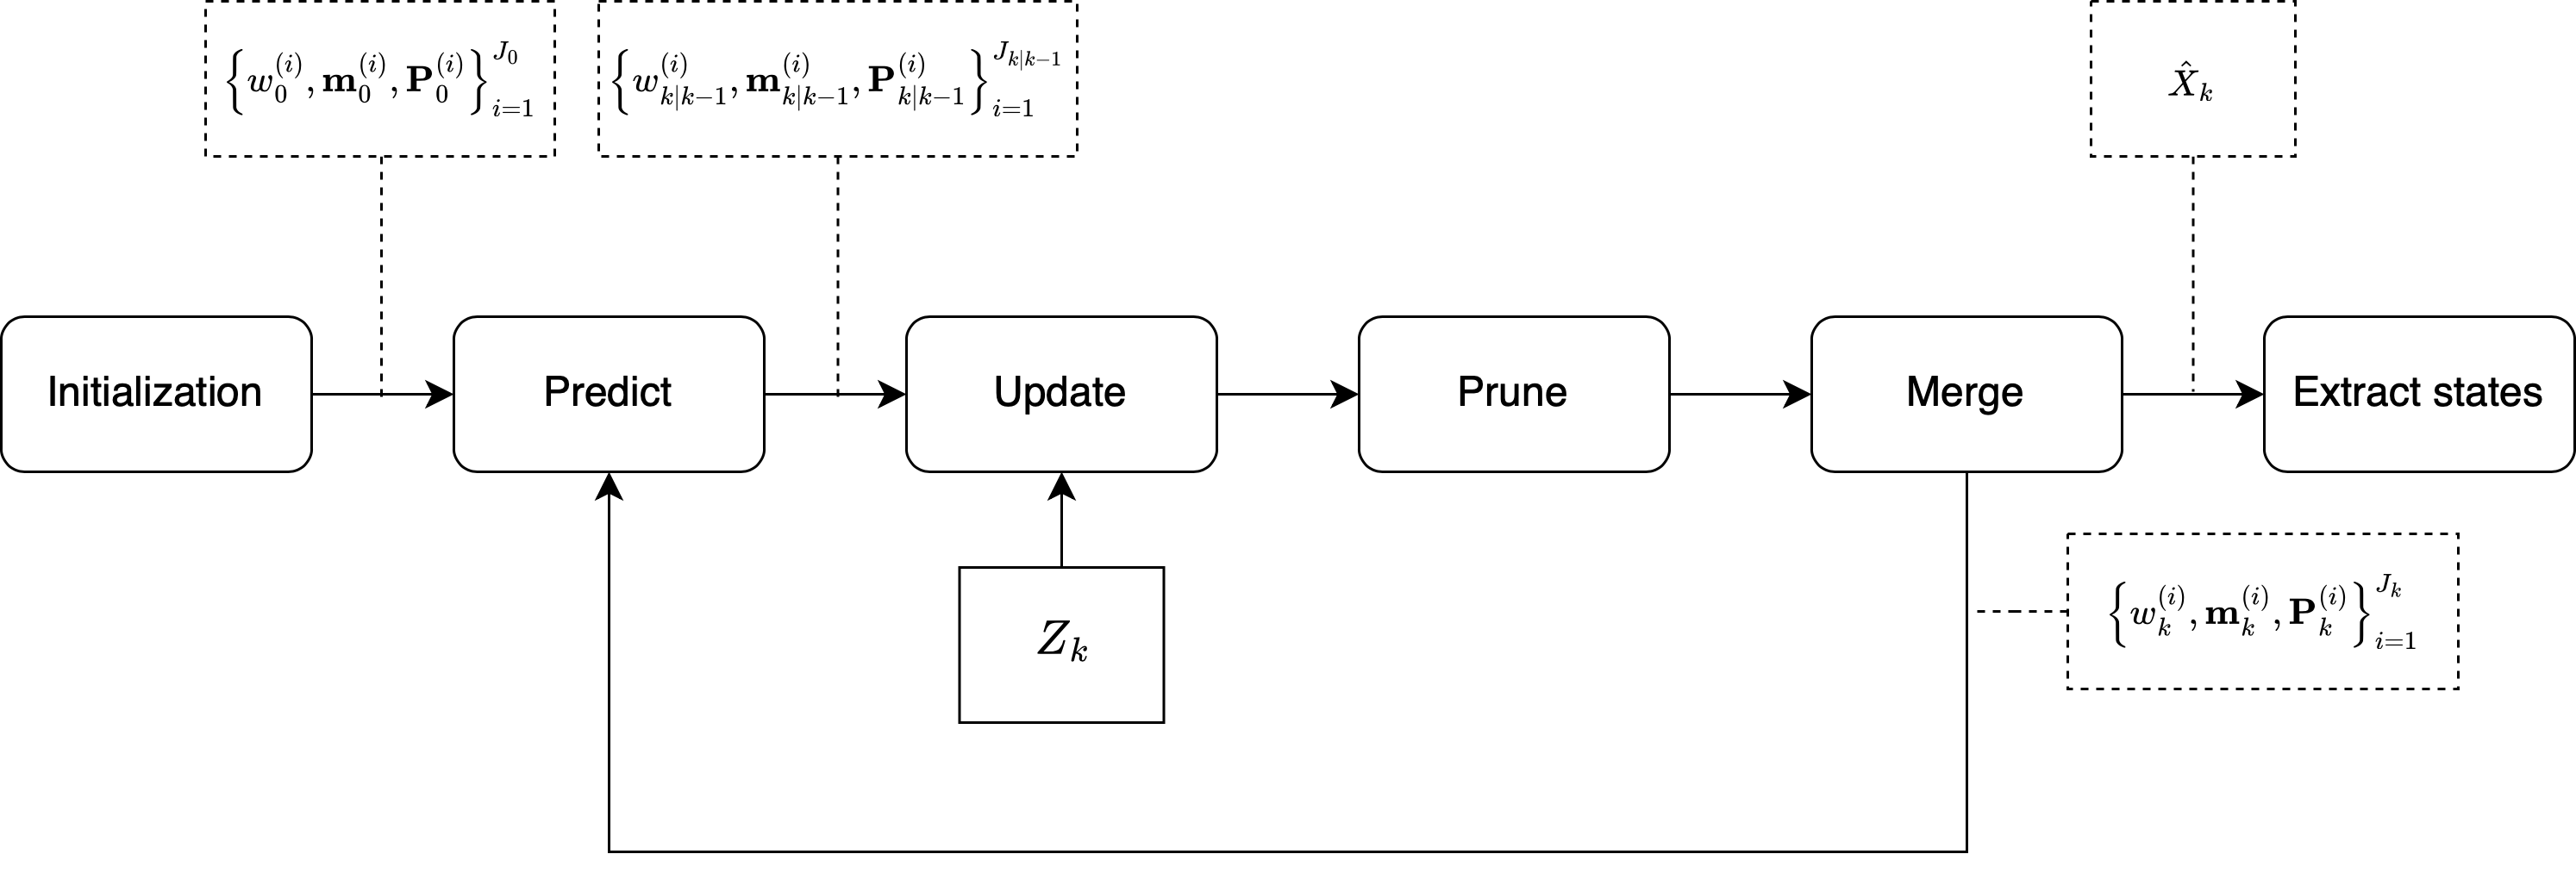
\includegraphics[width=.95\linewidth]{figures/gm-phd-cycle.png}
    \caption[GM-PHD Cycle.]{The visualization of the GM-PHD cycle.}
    \label{fig:gm-phd-cycle}
\end{figure}
